%%%%%%%%%%%%%%%%%%%%%%%%%%%%%%%%%%%%%%%%%%%%%%%%%%%%%%%%%%%%%%%%%%%%%%%%%%% 
% 
% Generic template for TFC/TFM/TFG/Tesis
% 
% By:
% + Javier Macías-Guarasa. 
% Departamento de Electrónica
% Universidad de Alcalá
% + Roberto Barra-Chicote. 
% Departamento de Ingeniería Electrónica
% Universidad Politécnica de Madrid   
% 
% Based on original sources by Roberto Barra, Manuel Ocaña, Jesús Nuevo,
% Pedro Revenga, Fernando Herránz and Noelia Hernández. Thanks a lot to
% all of them, and to the many anonymous contributors found (thanks to
% google) that provided help in setting all this up.
% 
% See also the additionalContributors.txt file to check the name of
% additional contributors to this work.
% 
% If you think you can add pieces of relevant/useful examples,
% improvements, please contact us at (macias@depeca.uah.es)
% 
% You can freely use this template and please contribute with
% comments or suggestions!!!
% 
%%%%%%%%%%%%%%%%%%%%%%%%%%%%%%%%%%%%%%%%%%%%%%%%%%%%%%%%%%%%%%%%%%%%%%%%%%% 

\chapter{Efficient Baselines for Multi-modal \\ Motion Prediction in Autonomous Driving}
\label{cha:efficient_baseline_for_mp_in_ad}

\begin{FraseCelebre}
	\begin{Frase}
		La fuerza de tus convicciones \\
		determina tu éxito, \\
		no el número de tus seguidores.
	\end{Frase}
	\begin{Fuente}
		Reamus Lupin \\
		Harry Potter y Las Reliquias de la Muerte, Parte 2
	\end{Fuente}
\end{FraseCelebre}

\section{Introduction}
\label{sec:6_introduction}

As observed in the previous Chapter, our \ac{GAN}-based model (more specifically the generator) was able to compute the deep context regarding the agents past observations, attention-based social interaction and target points as physical context, but the prediction was limited to the unimodal case. In other words, the \ac{GAN}-based model is able to reason more complex interactions and future behaviours than SmartMOT (physics-based prediction), but it lacks one of the main features of a deep learning-based model as a preliminary stage before the local planning or decision-making layers: Multimodality. On top of that, at this point of the thesis the literature was re-visited and despite \acp{GAN}-based approaches \cite{sadeghian2019sophie, dendorfer2020goal, gupta2018social, gomez2022exploring} provide certain control since they are focused on more simple methods framed in an adversarial training, most competitive approaches on \ac{MP} benchmarks in the field of \ac{AD}, such as Argoverse \cite{chang2019argoverse}, NuScenes \cite{caesar2020nuscenes} or Waymo \cite{ettinger2021large}, do not use adversarial training, where the training complexity is one the main reasons.

\begin{comment}
In this paper, following the same principles as recent SOTA methods, we aim to achieve competitive results that ensure reliable predictions, as observed in Fig.~\ref{fig:results_teaser}, yet, using \textbf{light-weight} attention-based models that take as input the past trajectories of each agent, and integrate prior-knowledge about the map easily. The main contributions of our work are as following: 

\begin{itemize}
	\item (1) Identify a key problem in the size of motion prediction models, with implications in real-time inference and edge-device deployment.
	\item (2) Propose several efficient baselines for vehicle motion prediction that do not explicitly rely on an exhaustive analysis of the context HD map (either vectorized or rasterized), but on prior map information obtained in a simple preprocessing step, that serves as a guide in the prediction.
	\item (3) Use fewer parameters and operations (FLOPs) than other SOTA models to achieve competitive performance on Argoverse 1.0~\cite{chang2019argoverse} with lower computational cost.
\end{itemize} 
\end{comment}

\section{Efficient Baselines}
\label{sec:6_efficient_baselines}

Considering the trade-off between curated input data and complexity, we aim to achieve competitive performance in the \ac{MP} using powerful DL techniques in terms of prediction metrics (\ac{minADE}, \ac{minFDE}), including attention mechanisms and \acp{GNN}, while reducing the number of parameters of operations with respect to other \ac{SOTA} methods. In particular, we propose two baselines, social and map baseline. 

The only inputs for the social baseline are the agent past trajectories and their corresponding interactions. On the other hand, for the map baseline, we propose an extension with respect to our previous target points proposals where, based on a simple-yet-powerful map pre-processing algorithm where the corresponding agent trajectory is initially filtered, the feasible area with which the agent can interact is computed. In spite the fact that topological, semantic and geometric information are involved while computing this area due to road connectivity, we only retrieve the geometric information of the feasible area proposals in an efficient and elegant way. Therefore, our models do not require full-annotated (including, topological, geometric and semantic) HD Map information as input or even rasterized \ac{BEV} representations of the scene to compute the physical context. Figure \ref{fig:chapter_6_Efficient_Baselines/TITS_2023} illustrates an overview of our final approach. We distinguish three main blocks: 1) \textbf{Encoding module}, which uses plausible HD Map information (specific centerlines and driveable area around) and agents past trajectories to compute the motion and physical latent features, 2) \textbf{Social Attention module}, which calculates the interaction among the different agents and returns the most relevant social features, 3) \textbf{Decoding module}, responsible for calculating the multimodal prediction by means of an auto-regressive strategy concatenating low-level map features and social features as a baseline, as well as iterating over the different latent centerlines for specific physical information per mode.



\begin{figure}[!h]
	\centering
	\setlength{\tabcolsep}{2.0pt}
	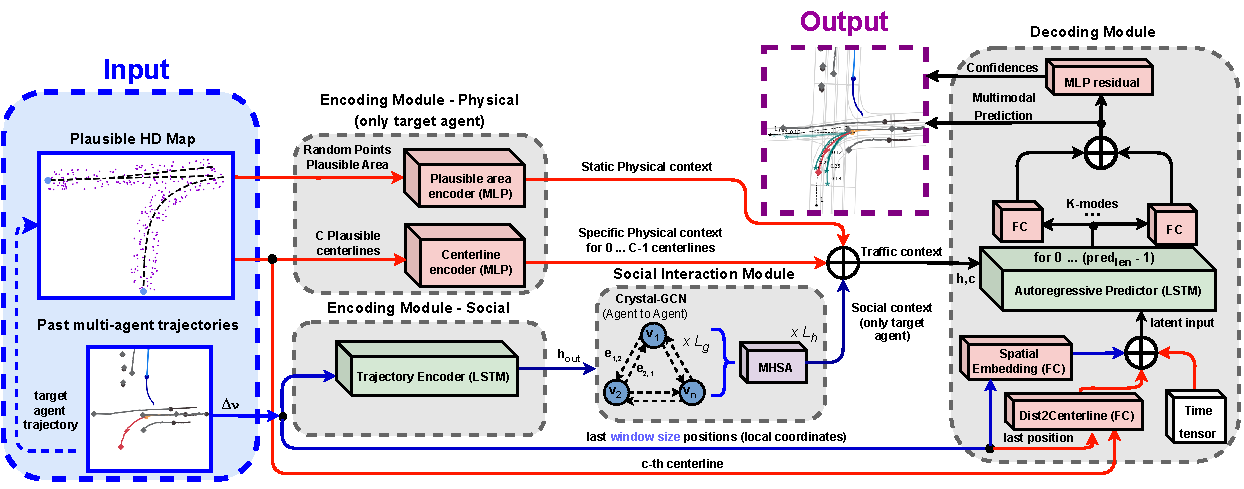
\includegraphics[width=0.95\linewidth]{chapter_6_Efficient_Baselines/TITS_2023.pdf}
	% \captionsetup{justification=justified}
	\caption[Overview of our Social and Map Efficient Baselines]{Overview of our Social and Map Efficient Baselines \\ (\textbf{\textcolor{blue}{Blue links}} and \textbf{\textcolor{red}{Red links}} represent \textbf{\textcolor{blue}{Social}} and \textbf{\textcolor{red}{Map}} information respectively).}
	\label{fig:chapter_6_Efficient_Baselines/TITS_2023}
\end{figure}

\subsection{Social Baseline}
\label{subsec:6_efficient_baselines_social}

Our social baseline is inspired in the architecture proposed by \cite{schmidt2022crat}. It uses as input the past trajectories of the most relevant obstacles as relative displacements to feed the Encoding Module (Figure \ref{fig:chapter_6_Efficient_Baselines/TITS_2023}). Then, the social information is computed using a \ac{GNN}, in particular Crystal-Graph Convolutional Network (\textbf{Crystal-GCN}) layers \cite{xie2018crystal, schmidt2022crat}, and Multi-Head Self Attention (MHSA) \cite{vaswani2017attention} to obtain the most relevant agent-agent interactions. Finally, we decode this latent information using an \textbf{autoregressive} strategy where the output at the \textit{i-th} step depends on the previous one for each mode respectively in the Decoding Module. The following sections provide in-depth description of the aforementioned modules.

\subsubsection{Preprocessing and Encoding of past trajectories}
\label{subsubsec:6_efficient_baselines_social_preprocessing_and_encoding}

In a similar way to the GAN-based model proposed in Chapter \ref{cha:exploring_gan_for_vehicle_mp}, in these efficient baselines we only consider the agents that have information over the full history horizon $T_h$ = \textit{$obs_{len}$} + \textit{$pred_{len}$}, reducing the number of agents to be considered in complex traffic scenarios. Nevertheless, instead of only substracting the origin of the scene (last position of the target agent) to make the model translation-invariant, we also rotate the whole coordinate system, \ie \ the coordinate system in our model is centered on the target agent at $t = 0$, and we use the orientation from the target location in the same timestamp as the positive $x$-axis. Note that this representation will benefit the model to have a common representation to enhance the generalization of the model and prevent over-fitting. Once the scene has been translated and rotated, instead of using absolute 2D-BEV (\textit{xy} plane), the input for the agent \textit{i} is a series of relative displacements.

Then, as stated in Chapter \ref{cha:exploring_gan_for_vehicle_mp}, we do not limit nor fix the number of agents per sequence, and a single \ac{LSTM}-based encoder computes the deep features of the motion history of the agents. Finally, in order to feed the agent-agent interaction module (Social Attention Module in Figure \ref{fig:chapter_6_Efficient_Baselines/TITS_2023}), we take the output hidden vector ($\mathbf{h_{out}}$).

\subsubsection{Social Attention module}
\label{subsubsec:6_efficient_baselines_social_interactions}

After encoding the past history of each vehicle in the sequence, we compute the agent-agent interactions to obtain the most relevant social information of the scene. For this purpose, we construct an interaction graph using Crystal-GCN \cite{xie2018crystal} \cite{schmidt2022crat}. , originally developed for the prediction of material properties, allowing to efficiently leverage edge features. Then, \ac{MHSA} \cite{vaswani2017attention} is applied to enhance the learning of agent-agent interactions. 

Before creating the \textbf{interaction mechanism}, we split the temporal information in the corresponding scenes, taking into account that each traffic scenario may have a different number of agents. The interaction mechanism is defined in \cite{schmidt2022crat} as a bidirectional fully-connected graph, where the initial node features $\mathbf{v}_i^{(0)}$ are represented by the latent temporal information for each vehicle $\mathbf{h}_{i,out}$ computed by the motion history encoder. On the other hand, the edges from node \textit{k} to node \textit{l} is represented as the vector distance ($\mathbf{e}_{k,l}$) between the corresponding agents at t = \textit{$obs_{len}$} in absolute coordinates, where the origin of the sequence ($x=0,y=0$) is represented by the position of the target at t = \textit{$obs_{len}$}:

\begin{equation}
	\mathbf{e}_{k,l} = \boldsymbol{\nu}^{obs_{len}}_k - \boldsymbol{\nu}^{obs_{len}}_l \text{,}
\end{equation}

Given the interaction graph (nodes and edges), the Crystal-GCN, proposed by \cite{xie2018crystal}, is defined as:

\begin{equation}
	\mathbf{v}_i^{(g+1)} = \mathbf{v}_i^{(g)} +
	\sum_{j = 0 \textbf{:} j \neq i }^{N} \sigma \left( \mathbf{z}_{i,j}^{(g)} \mathbf{W}_\mathrm{f}^{(g)} + \mathbf{b}_\mathrm{f}^{(g)} \right)
	\odot \mu \left( \mathbf{z}_{i,j}^{(g)} \mathbf{W}_\mathrm{s}^{(g)} + \mathbf{b}_\mathrm{s}^{(g)}  \right)
\end{equation}

This operator, in contrast to many other graph convolution operators \cite{zeng2021lanercnn} \cite{liang2020learning}, allows the incorporation of edge features in order to update the node features based on the distance among vehicles (the closer a vehicle is, the more is going to affect to a particular node). As stated by \cite{schmidt2022crat}, we use $L_g = 2$ layers of the GNN ($g \in 0, \dots , L_g$ denotes the corresponding Crystal-GCN layer) with ReLU and batch normalization as non-linearities between the layers. $\sigma$ and $\mu$ are the sigmoid and softplus activation functions respectively. 

Moreover, $\mathbf{z}_{i,j}^{(g)} = ( \mathbf{v}_i^{(g)} || \mathbf{v}_j^{(g)} ||\mathbf{e}_{i,j} )$ corresponds to the concatenation of two node features in the \textit{$g_{th}$} GNN layer and the corresponding edge feature (distance between agents), N represents the total number of agents in the scene and $\mathbf{W}$ and $\mathbf{b}$ the weights and bias of the corresponding layers respectively.

After the interaction graph, each updated node feature $\mathbf{v}_i^{(L_g)}$ contains information about the temporal and social context of the agent \textit{i}. Nevertheless, depending on their current position and past trajectory, an agent may require to pay attention to specific social information. To model this, we make use of a scaled dot-product Multi-Head Self-Attention mechanism \cite{vaswani2017attention} which is applied to the updated node feature matrix $\mathbf{V}^{(L_g)}$ that contains the node features $\mathbf{v}_i^{(L_g)}$ as rows. 

Each head $h \in 1,\dots, L_h$ in the MHSA mechanism is defined as:

\begin{equation}
	\mathrm{head}_h = \mathrm{softmax} \left( \frac{\mathbf{V}^{(L_g)}_{Q_h} \mathbf{V}^{(L_g) T}_{K_h}}{\sqrt{d}}  \right) \mathbf{V}^{(L_g)}_{V_h} \text{.}
\end{equation}

where $\mathbf{V}^{(L_g)}_{Q_h}$ (Query), $\mathbf{V}^{(L_g)}_{K_h}$ (Key) and $\mathbf{V}^{(L_g)}_{V_h}$ (Value) represent the \textit{$h_{th}$} head linear projections of the node feature matrix $\mathbf{V}^{(L_g)}$ and $d$ is the normalization factor corresponding to the embedding size of each head. For our purpose, we use $L_h = 4$ as the total number of heads. 

The result of the softmax weights multiplied by the node feature matrix $\mathbf{V}^{(L_g)}_{V_h}$ (Value) is often referred as the attention weight matrix, representing in this particular case pairwise dependencies among vehicles.

Finally, the updated node feature matrix $\mathbf{SATT}$ is computed as the combination of the different attention heads in a single matrix:

\begin{equation}
	\mathbf{SATT} = (\mathrm{head}_1 || \dots || \mathrm{head}_{L_h}) \mathbf{W}_\mathrm{o} + 
	\begin{pmatrix}
		\mathbf{b}_\mathrm{o}\\
		\vdots \\
		\mathbf{b}_\mathrm{o}
	\end{pmatrix}.
\end{equation}

Where each row of the final social attention matrix $\mathbf{SATT}$ (output of the social attention module, after the GNN and MHSA mechanisms) represents the interaction-aware feature of the agent \textit{i} with surroundings agents, considering the temporal information under the hood, being $\mathbf{W}_\mathrm{o}$ / $\mathbf{b}_\mathrm{o}$ the corresponding weight and bias of the layer that merges the different attention heads. As this model has been developed upon the Argoverse 1 Motion Forecasting benchmark, we only consider the row of the final matrix that takes into account the interactions of the target agent with surrounding obstacles.

\subsection{Map Baseline} 
\label{subsec:6_efficient_baselines_map_baseline}

As mentioned before, in this work we extend our social baseline using minimal HD map information, from which we discretize the feasible area $\mathcal{P}$ of the target agent as a subset of $r$ randomly sampled points $\{p_0 , p_1 ... p_r\}$ (low-level features) around the plausible centerlines (high-level and well-structured features) considering the velocity and acceleration of the corresponding agent in the last observation frame, as observed in Figure \ref{fig:chapter_6_Efficient_Baselines/efficient_baselines_hdmap_filtering}. As stated in Section \ref{sec:5_attention_gan}, this is a map preprocessing step, therefore the model never sees the HD map (either vectorized or rasterized) image nor the whole graph of nodes.

\subsubsection{Centerlines proposals and Feasible area points} 
\label{subsubsec:6_efficient_baselines_preprocessing_map}

In a similar way to the target points computed in our \ac{GAN}-based model, we want to compute the heuristic proposals for each agent. Nevertheless, instead of limiting the map baseline to some discrete target points, now we aim to compute the most plausible future centerlines (that is, the center of the lane) as a connection of nodes (waypoints). Considering lane connectivity, multiple approaches have tried to predict realistic trajectories by means of learning physically feasible areas as heatmaps or probability distributions of the agent’s future location~\cite{dendorfer2020goal, sadeghian2019sophie, gilles2021home}. \cite{liang2020learning} represents the map as a set of lanes and their connectivity (predecessor, successor, right neighbour, left neighbour), taking into account all lanes whose distance from the target agent is smaller than 100 m as the input, regardless the orientation or the velocity of the vehicle. On the other hand, \cite{djuric2021multixnet} encodes static elements such as crosswalks, lane, road boundaries and intersections that are included in a local map 150m x 100m centered in the corresponding vehicle  as a multi-channel image.  These approaches require either a top-view RGB \ac{BEV} image of the scene, or a HD map with exhaustive topological, geometric and semantic information (commonly codified as channels). This information is usually encoded using a \ac{CNN} and fed into the model together with the social agent's information \cite{dendorfer2020goal, sadeghian2019sophie, gao2020vectornet}. 

As observed, when trying to utilize HD map information, specially in terms of lane proposals, most SOTA methods utilize this physical to enhance the latent information to decode the future trajectories, but heavy computation or raw data features are required. 

\begin{figure*}[]
	\centering
	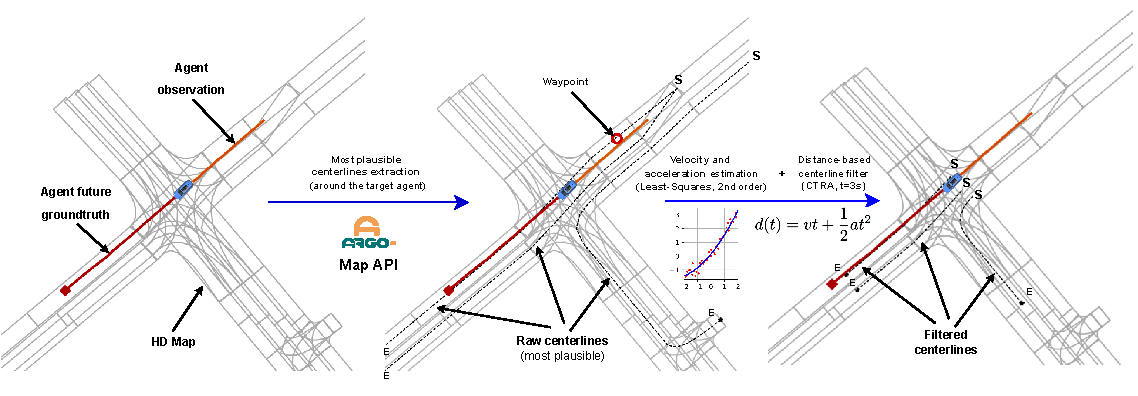
\includegraphics[width=0.95\linewidth]{chapter_6_Efficient_Baselines/compute_centerlines_argo_1.pdf}
	\captionsetup{justification=justified}
	\caption[Plausible centerlines estimation in Argoverse 1]{Plausible centerlines estimation. Left: General view of the scene, only considering the target agent (\textbf{\textcolor{YellowOrange}{observation (2s)}} and \textbf{\textcolor{red}{future ground-truth (3s)}}) and HD Map around its last observation (position of the \textbf{\textcolor{blue}{blue}} vehicle). Center: \textbf{Centerlines} proposed by the Argoverse Map API (maximum number of centerlines \textit{C} set to 3). Right: We filter the input observation by means of Least-Squares (2nd order) algorithm to estimate the velocity and acceleration of the agent. Then, the distance considering the \ac{CTRA} model and a prediction horizon of 3 s are used computed to obtain the end-points \textbf{E} of the \textbf{final proposals}. Start-points \textbf{S} are the closest centerlines waypoints to the agent in the last observation frame.}
	\label{fig:chapter_6_Efficient_Baselines/efficient_baselines_hdmap_filtering}
\end{figure*}

\textbf{Effectively} and \textbf{efficiently} exploiting HD maps is a must for MP models to produce accurate and plausible trajectories in real-time applications, specially in the field of AD, providing specific map information to each agent based on its kinematic state and geometric HD map information. In that sense, we propose to obtain the most plausible \textit{M} lane candidates, we make use of the pertinent heuristic functions proposed by the Argoverse 1 Motion Forecasting dataset Map API \cite{chang2019argoverse} as illustrated by \cite{khandelwal2020if} to choose the closest centerlines to the last observation data of the target agent, which are going to represent its most representative future trajectories. On the other hand, as depicted in the \ac{MP} dataset used to train this model (Argoverse 1), vehicles are the only evaluated object category as the target agent. Then, considering a vehicle as a rigid structure with non-holonomic \cite{triggs1993motion} features (no abrupt motion changes between consecutive timestamps) and the road driving task is usually described as anisotropic \cite{ross1989planning} (most relevant features are found in a specific direction, in this case the lanes ahead). In other words, the agent should follow a smooth trajectory in a short-mid term prediction. The heuristic to obtain these centerlines is summarized as follows:

\begin{enumerate}
	\item Trajectory data presents noise associated to the real-world data capturing the exact position of the previously tracked vehices in real-world scenarios. Regarding this, we filter the agent trajectory as a polynomial curve fitting problem by means of the Least Squares ($2^{nd}$ order) per axis and Savitzky-Golais \cite{savitzky1964smoothing} algorithms to obtain a smooth representation of the position vector.
	
	\item By doing so, and assuming the agent is moving with a constant acceleration, we are able to calculate the subsequent derivatives (velocity and acceleration) of the target agent in $t_{obs_{len}}$. Then, a vector of $obs_{len}$ - 1 and $obs_{len}$ - 2 length is computed to estimate the velocity and acceleration respectively as $V_{i}=\frac{X_{i}-X_{i-1}}{t_{i}-t_{i-1}}$ and $A_{i}=\frac{V_{i}-V_{i-1}}{t_{i}-t_{i-1}}$, where $X_{i}={[x_{i},y_{i}]}$ represents the 2D position of the agent at each observed frame $i$.
	
	\item In order to compute the velocity, acceleration and yaw angle in the last observation frame, we compute a weighted mean by assigning less importance (weight) to the first positions of the corresponding vector and higher importance to the latter states, in such a way immediate past observations are the key states to determine the current spatio-temporal variables of the agent, as depicted in Equation \ref{eq:5_dynamic_feats_last_observation_frame}.
	
	\item We compute the future travelled distance by means of the well-known Constant Acceleration (CA) model:
	
	\begin{equation}
		d(t) = x_0 + vt + \frac{1}{2}at^2
	\end{equation}
	
	where $t$ corresponds to the prediction horizon $pred_{len}$, $x_0$ is equal to $0$ since we want to determine the travelled distance from the current position and $v$ and $a$ are the velocity and acceleration in the last observation frame previously calculated. Note that we assume that this is a \ac{CTRA} model, instead of only \ac{CA} in a specific direction, since the orientation is implicit in the lane boundaries. That's why it does not make sense to involve the orientation at frame $t=0$ in the travelled distance calculation.
	
	\item Get all lane candidates within a bubble, given the agent last observation and Manhattan distance.
	
	\item Expand the bubble until at least 1 lane is found.
	
	\item Once some preliminary proposals are found, we employ the Depth First Search (DFS) algorithm to get all successor and predecessor candidates, merging the past and future candidates and removing the overlapping ones.
	
	\item Then, we process these raw candidates so as to use them as plausible physical information. Given these raw lanes, we aim to limit the number of centerlines to a fixed number $M$. First, given the previously computed smoothed trajectory, we compute the closest centerlines to our current position since they will represent the most realistic future lanes in the traffic scenario. Second, we evaluate the above-mentioned travelled distance along the raw centerlines. We determine the end-point index $p$ of the centerline $m$ as the waypoint (each discrete node of the centerline) where the accumulated distance (considering the $\mathcal{L}_2$ distance between each waypoint) is greater or equal than the above-computed $d(obs_{len})$:
	
	\begin{equation}
		p \quad \textbf{:} \quad d(obs_{len}) \leq \sum_{p=start_{point}}^{centerline_{length}} \mathcal{L}_2(w(p+1),w(p))
	\end{equation}
	
	\item Finally, in order to have the same points (particularly, the number of points matches the prediction horizon $pred_{len}$) per centerline, we interpolate them using a $1^{st}$ spline order, considering as start point the last agent observation and as end or goal point the aforementioned travelled distance along the corresponding centerline.
	
	\item Note that if the number of proposed centerlines is lower than a pre-defined number $M$, a virtual centerline is created and padded with zeros.
\end{enumerate}

Figure \ref{fig:chapter_6_Efficient_Baselines/efficient_baselines_hdmap_filtering} summarizes this HDMap filtering process, where we are able to estimate the preliminary centerlines proposals as a \textbf{simplified version of the HD map}. Moreover, Fig. \ref{fig:chapter_6_Efficient_Baselines/efficient_baselines_hdmap_filtered_examples} illustrates how after our filtering process the end-points of the plausible centerlines are noticeable closer to the ground-truth prediction at the final timestep. 

In addition to these \textbf{high-level} and well-structured centerlines, we apply point location perturbations to all plausible centerlines under a $\mathcal{N}(\mu, \sigma)$ [m] distribution~\cite{ye2021tpcn} in order to discretize the plausible area $\mathcal{P}$ as a subset of $r$ randomly sampled points $\{p_0 , p_1 ... p_r\}$ (\textbf{low-level} features) around the plausible centerlines. By doing this, we may have a common representation of the plausible area, defined as low-level map features. We make use of a normal distribution $\mathcal{N}$ to calculate these random points as an additional regularization term in a similar way that data augmentation is applied to the past trajectories. 

\begin{figure}[t!]
	\begin{subfigure}{0.5\textwidth}
		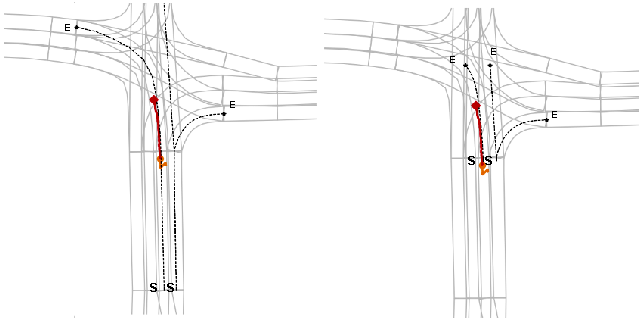
\includegraphics[width=\textwidth]{chapter_6_Efficient_Baselines/compute_centerlines_example_1.pdf}
		
	\end{subfigure}
	\hfill
	\begin{subfigure}{0.5\textwidth}
		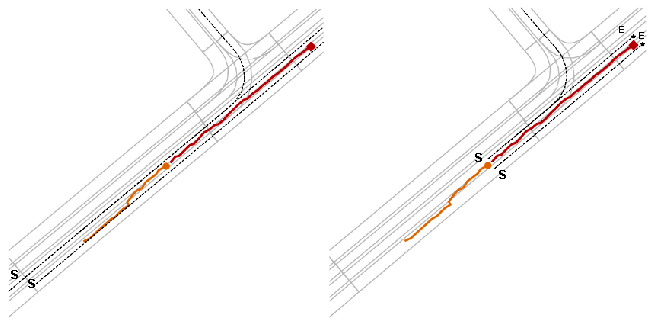
\includegraphics[width=\textwidth]{chapter_6_Efficient_Baselines/compute_centerlines_example_2.pdf}
		
	\end{subfigure}
	
	\captionsetup{justification=justified}
	\caption[Some challenging examples of our preprocessing step to obtain relevant map features]{Some challenging examples of our preprocessing step to obtain relevant map features. In both scenarios the target agent (\textbf{\textcolor{YellowOrange}{observation (2 s)}} and \textbf{\textcolor{red}{future ground-truth (3 s)}}) presents a noticeable noisy past trajectory and the provided raw \textbf{centerlines} do not consider the current kinematic state of the vehicle. (a) The agent is stopped (maybe due to an stop, pedestrian crossing or red traffic light use case). We estimate a minimum travelled distance of 25 m in these situations to determine the centerline end-points \textbf{E}. (b) In this scenario, we can observe how the raw centerlines consider way more distance (both ahead and behind) than required. Our kinematic-based filter is able to minimize these proposals in an interpretable way to serve as prior information to the MP model
	}
	\label{fig:chapter_6_Efficient_Baselines/efficient_baselines_hdmap_filtered_examples}
\end{figure}

\subsubsection{Encoding module of map information}
\label{subsubsec:6_efficient_baselines_encoding_map}

In order to calculate the latent map information, we employ a plausible area and centerline encoder (Figure \ref{fig:chapter_6_Efficient_Baselines/TITS_2023}) to process the low-level and high-level map features respectively. Each of these encoders are represented by a Multi-Layer Perceptron (MLP). First, we flat the information along the points dimension, alternating the x-axis and y-axis information. Then, the corresponding MLP (three layers, with batch normalization, interspered ReLUs and dropout in the first layer) transforms the interpretable absolute coordinates around the origin ($x=0, y=0$) into representative latent physical information. The static physical context (output from the plausible area encoder) will serve as a common latent representation for the different modes, whilst the specific physical context will illustrate specific map information for each mode.

\subsection{Augmented Efficient baseline with Transformer Encoders}
\label{subsec:6_augmented_baseline}

Once the social and map baseline encoders are stated, we focus on a more powerful mechanism to encode the spatial and temporal information of inputs by encoding them into feature vectors. In that sense, we focus of designing an effective encoder transformer while keeping its structure as simple and efficient as possible. In a similar way to \cite{wang2023lane}, we adopt the combination of CNN/MLP, attention block and normalization, as observed in Figure \ref{fig:chapter_6_Efficient_Baselines/ITSC_2023}.

\begin{figure*}[!ht]
	\centering
	\setlength{\tabcolsep}{2.0pt}
	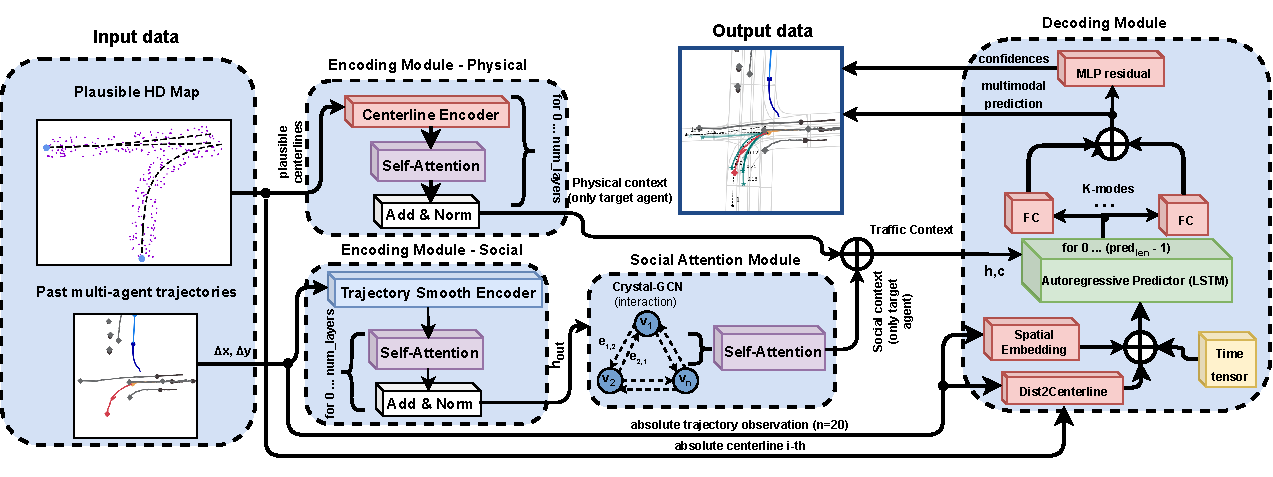
\includegraphics[width=0.95\linewidth]{chapter_6_Efficient_Baselines/ITSC_2023.pdf}
	\caption{Efficient baseline with transformer encoders to process the physical and social input}	
	\label{fig:chapter_6_Efficient_Baselines/ITSC_2023}
\end{figure*}

In order to encode the centerlines, we first use an MLP-based encoder to transform the input vector at each time stamp ($d_i^t$, which actually represents a plausible position of the target agent) into deep features:

\begin{equation}
	f_i^t=MLP_{\text{map}}\left(d_i^t ; W_{\text {map }}\right)
\end{equation}

where $MLP_{\text{map}}$ is a Multi-Layer (3) Perceptron with a ReLU asnon-linear layer and $W_{\text {map }}$ as the weight matrix that is learnable. However, to predict the future trajectory, the separate feature of each vector is insufficient. For example, even if two road segments in the first half have the same structure, the difference in the last half can result in a total difference in geometric meaning. Therefore, we make use of the well-established Multi-Head Self-Attention (MHSA) \cite{vaswani2017attention} mechanism to encode the overall set of physical features per agent as a single vector.

To be more specific, we first calculate the query, key and value matrix:

\begin{equation}
	q_i^t=W^q f_i^t, k_i^t=W^k f_i^t, v_i^t=W^q f_i^t,
\end{equation}

where $W^q, W^k, W^v$ are the learnable weight matrices. Then, we take these three matrices as the inputs of the weighting block based on softmax:

\begin{equation}
	h_i^t=\operatorname{softmax}\left(\frac{q_i^t \cdot k_i^{t T}}{\sqrt{d_k}}\right) v_i^t,
\end{equation}

where $d_k$ is the length of matrix $k$. Finally, we adopt a 2-layer MLP to aggregate the features of vectors within a road segment:

\begin{equation}
	h_i=MLP_{a g g}\left(h_i^t ; W_{a g g}\right)
\end{equation}

where $MLP_{a g g}$ is a 2-layer MLP with a ReLU non-linear layer and $W_{a g g}$ is the weight matrix that is learnable. Now, we have the feature vector for each target agent, stored as a 2D matrix $(M, H)$, where $M$ is the number of road segments and $\mathrm{H}$ is the length of hidden features. 

For agents, we use similar techniques to encode and aggregate the information. In particular, we use a trajectory encoder block to encode each vector into the form of a feature vector. Then, similar to roads, even two vehicles have the same movement in the first half of their trajectory, and the differences in the last half of trajectories can lead to a totally different future trajectory. Therefore, we use a MHSA block to encode the overall feature of one trajectory in the observed time period and form a single feature vector for each agent. Finally, a 2-layer MLP-based aggregator is used to construct a single feature vector for each trajectory.

One aspect worth mentioning is the agent encoder. While trajectory data are, unlike roads (well structured) usually non-smooth, as expected from real-world datasets. Then, while we make use of MLP to compute the deep physical features, we use a 1D-CNN based motion encoder in the first stage due to its wider receptive field compared with MLP in such a way the convolutional encoder can smooth the trajectories and reduce the influence of noisy input trajectories.

\subsection{Decoding module}
\label{subsubsec:6_efficient_baselines_decoding_modules}

The decoding module is the third component of our baselines, as observed in Figure \ref{fig:chapter_6_Efficient_Baselines/TITS_2023}. The decoding module consists of an \textbf{LSTM} network, which recursively estimate the relative displacements for the future timesteps, in the same way we studied the past relative displacements in the Motion History encoder. Regarding the social baseline, the model uses the social context computed by the Social Interaction Module, only paying attention to the target agent row. Then, only the social context corresponds to the whole \textit{traffic context} of the scenario, representing the input hidden vector of the autoregressive LSTM predictor. On the other hand, in terms of the map baseline, for a mode \textit{k}, we identify the latent \textit{traffic context} as the concatenation of the social context, static physical context and specific physical context as stated in Section \ref{subsubsec:6_efficient_baselines_encoding_map}, which will serve as input hidden vector $\mathbf{h}$ of the LSTM decoder. In both cases (social and map baselines), the cell vector $\mathbf{c}$ is initialized with a vector of zeros of the same dimension. 

Regarding the LSTM input, in the social case it is represented by the encoded past $n$ relative displacements of the target agent after a spatial embedding, whilst the map baseline adds the encoded vector distance between the current absolute target position and the current centerline, as well as the current scalar timestamp $t$, as illustrated in Figure \ref{fig:chapter_6_Efficient_Baselines/TITS_2023}. In both cases (social and map baselines), we process the output of the LSTM using a standard Fully-Connected (FC) layer (one per mode). Once we have the relative prediction in the timestep $t$, we shift the initial past observation data in such a way we introduce our last-computed relative displacement at the end of the vector, removing the first data. We identify this technique as a \textit{temporal decoder}, where a window of size $n$ is analized by the autoregressive decoder in contrast to other techniques \cite{dendorfer2020goal, sadeghian2019sophie, gupta2018social} where only the last data is considered. Finally, after performing relative displacements to absolute coordinates operation, we obtain our multimodal predictions $\hat{Y} \in \mathbb{R}^{k \times pred_{len} \times data_{dim}}$, where $k$ represents the number of modes, $pred_{len}$ represents the prediction horizon and $data_{dim}$ represents the data dimensionality, in this case $xy$, predictions from the BEV perspective). Once the multimodal predictions are computed, they are concatenated and processed by a residual MLP to obtain the confidences (the higher the confidence, the most probable the mode must be, and closer to the ground-truth).

\subsection{Losses}
\label{subsec:6_efficient_baselines_losses}

We use the standard \textbf{Negative Log-Likelihood} (NLL) loss to train our social and map baselines in order to compare the ground-truth points $Y \in \mathbb{R}^{pred_{len} \times data_{dim}} = \{(x_0,y_0) ... (x_{pred_{len}}, y_{pred_{len}})\}$ with our multimodal predictions ($\hat{Y} \in \mathbb{R}^{k \times pred_{len} \times data_{dim}}$), given $k$ modalities (hypotheses) $\mathbf{p}=\{(\hat{x}^1_0,\hat{y}^1_0) ... (\hat{x}^k_{pred_{len}}, \hat{y}^k_{pred_{len}})\}$, with their corresponding confidences $\mathbf{c}=\{c_1 ... c_k\}$ using the following equation:

\begin{equation}
	\text{NLL} = -\log \sum_{k} e^{ \log{c^k} - \frac{1}{2} \sum_{t=0}^{pred_{len}} (\hat{x}^k_t - x_t)^2 + (\hat{y}^k_t - y_t )^2 }
	\label{eq:nll}
\end{equation}

Similar to \cite{mercat2020multi}, we assume the ground-truth points to be modeled by a mixture of multi-dimensional independent Normal distributions over time (predictions with unit covariance). Minimizing the NLL loss maximizes the likelihood of the data for the forecast. Nevertheless, the NLL loss tends to overfit most predictions in a similar direction. As stated above, in the motion prediction task, specially in the Autonomous Vehicles field, we must build a model that not only reasons multimodal predictions in terms of different maneuvers (keep straight, turn right, lane change, etc.) but also different velocity profiles (constant velocity, acceleration, etc.) regarding the same maneuver. For this reason, after the baselines models have been trained, as stated by \cite{kim2022improving}, we add as regularization the Hinge (\aka max-margin) and \textbf{Winner-Takes-All} (WTA) \cite{liang2020learning, kim2022improving} losses to improve the confidences and regressions respectively. 

Algorithm \ref{alg:6_efficient_baselines_additional_regularization} illustrates how we compute the max-margin and WTA losses. First, we determine the closest mode $m^{*}$ to the ground-truth using the $\mathcal{L}_2$ distance, only considering the end-points. Then, WTA loss is computed using Smooth~$\mathcal{L}_1$ distance taking into account in this case the whole prediction horizon between the best mode and ground-truth prediction. Finally, we apply the max-margin loss regarding the confidence of the best mode and a margin ($\epsilon$).

\begin{algorithm}[H]
	\SetAlgoLined
	\caption{Additional regularization: Hinge and WTA loss}
	\label{alg:6_efficient_baselines_additional_regularization}
	
	\SetKwInput{Input}{input}
	\SetKwInput{Output}{output}
	
	\Input{ground-truth trajectory $(Y \in \mathbb{R}^{pred_{len} \times data_{dim}})$ and output trajectories ($\hat{Y} \in \mathbb{R}^{k \times pred_{len} \times data_{dim}}$), where $k$, $pred_{len}$, and $data_{dim}$ denote the number of modes, prediction horizon, and data dimensionality for the target agent.}
	
	\Output{classification loss $\mathcal{L}_{Hinge}$ and regression loss $\mathcal{L}_{WTA}$}
	
	\For{$m$ in $\{1, 2, \ldots, k\}$}{
		$d_{wta}^m \gets$ Euclidean distance between $\hat{Y}^{m}_{pred_{len}}$ and $Y_{pred_{len}}$\;
	}
	
	$m^* = \arg\min_{m} d_{wta}^{m}$\;
	$\mathcal{L}_{reg,WTA} \gets $ Smooth $\mathcal{L}_1$ loss between $\hat{Y}^{m^*}$ and $Y$\;
	$\mathcal{L}_{class,Hinge} = \frac{1}{(K-1)}\sum_{m=1 \setminus m \neq m^*}^{K} \max( 0, c_{k} + \epsilon - c_{m^*})$\;
	
	\Return $\mathcal{L}_{WTA}$, $\mathcal{L}_{Hinge}$\;
	
\end{algorithm}

Therefore, our loss function is:

\begin{equation}
	\mathcal{L} = \alpha \mathcal{L}_{NLL} + \beta \mathcal{L}_{Hinge} + \gamma \mathcal{L}_{WTA}
	\label{eq:loss}
\end{equation}

\section{Experimental Results}
\label{sec:6_experimental_results}

\subsection{Implementation details}
\label{subsec:6_implementation_details}

To validate these efficient baselines (social, map and augmented baseline), we use the Argoverse 1 Motion Forecasting, as discussed in Section \ref{subsec:5_dataset}. In terms of evaluation metrics, we evaluate the performance of our models using the standard metrics \ac{ADE} and \ac{FDE}. Unlike the \ac{GAN}-based model, the output of the models in this Chapter is multimodal, then we generate $k$ outputs (also known as modes) per prediction step and report the metrics for the best out of $k$ outputs, regarding the agent $i$.

We report results for $k=1$ (unimodal case, only the mode with the best confidence is considered) and $k=6$ as this is the standard in the Argoverse Motion Forecasting dataset in order to compare with other models.

We train our models to convergence using a single NVIDIA RTX 3090, and validate our results on the official Argoverse 1 validation set~\cite{chang2019argoverse}. We use Adam optimizer with learning rate $0.001$ and default parameters, batch size $1024$ and linear LR Scheduler with factor $0.5$ decay on plateaus. We rotate the whole scene regarding the orientation in the last observation frame of the target agent to align this agent with the positive y-axis. The hidden dimension for the Motion History encoder is 64, where both the hidden state $\mathbf{h_{in}}$ and cell state $\mathbf{c_{in}}$ are initialized with zeros (dim = $128$), whilst the MLP encoder for both the specific centerline and plausible area is 128. Regarding the Social Interaction module, the latent vector of the Crystal-GCN layers is 128 and the number of heads in the MHSA module is $L_h = 4$. In terms of the Autoregressive predictor, the spatial embedding and \textit{dist2centerline} modules encode the past data and distance to the specific centerline using a \textit{window size} of 20. We set the number of plausible centerlines (\textit{M}) as 3, which cover most cases (if less than 3 plausible centerlines are available, we add padded centerlines as vector of zeros). The time tensor is a single number that represents the current timestep, in such a way the LSTM input is \textit{(2 $\times$ window size) + 1 = 41}. The regression head is represented by \textit{k=6} FC layers that map the output latent vector returned by the LSTM to the final output relative displacements (dim = 2, xy). Multimodal predictions are processed by an MLP residual of sizes 60, 60 and 6 with interspersed ReLU activations in order to obtain the corresponding confidences.

In terms of data augmentation, we make use of (i) Dropout and swapping random points from the past trajectory, (ii) point location perturbations under a $\mathcal{N}(0, 0.2)$ [m] noise distribution~\cite{ye2021tpcn}. We also apply the well-established hard-mining technique to improve the model generalization under difficult scenarios. To perform this technique, once we have the social and map baselines, we perform inference on the training set to find the most difficult scenes in terms of \ac{minADE}. Then, we mine those scenes such that the baselines models perform poorly, and increase their proportion in the batch during training.

\subsection{Model results}
\label{subsec:6_model_results}

\begin{table}[thpb]
	\captionsetup{justification=justified}
	\caption[Ablation Study for map-free MP on the Argoverse 1 validation set]{Ablation Study for map-free MP on the Argoverse 1 validation set. Our methods are indicated with $\dag$, our highlighted method indicates our map-free baseline (Best Social Model = BSM). Prediction metrics (minADE, minFDE) are reported in meters.}
	\label{table:results_val_social}
	% \setlength{\tabcolsep}{5pt}
	\centering
	\resizebox{\linewidth}{!}{
	\begin{tabular}{lccccc}
		\toprule
		\multirow{2}{*}{Method} & \multirow{2}{*}{Number of Parameters} &
		\multicolumn{2}{c}{$k=1$} & \multicolumn{2}{c}{$k=6$} \\ 
		& & minADE & minFDE & minADE & minFDE  \\ 
		\midrule
		TPCN \cite{ye2021tpcn} & - & 1.42 & 3.08 & 0.82 & 1.32 \\
		LaneGCN  \cite{liang2020learning} (w/o map) & $\approx 1 M $ & 1.58 & 3.61 & 0.79 & \textbf{1.29} \\
		WIMP \cite{khandelwal2020if} (w/o map) & $> 20 M$ & $1.61$ & 5.05 & 0.86 & 1.39 \\
		CRAT-Pred (LSTM + GNN + Lin. Residual) \cite{schmidt2022crat} & 449K & 1.44 & 3.17 & 0.86 & 1.47 \\
		CRAT-Pred (LSTM + GNN + Multi-Head Self-Attention + Lin. Residual) \cite{schmidt2022crat} & 515K & \textbf{1.41} & \textbf{3.10} & 0.85 & 1.44 \\ 
		\midrule
		$\dag$ LSTM-128 + GNN + MHSA (Baseline social) &  351K  & 1.82 & 3.72 & 0.87 & 1.63 \\
		$\dag$ LSTM-64 + GNN + MHSA &  \textbf{97K}  & 1.77 & 3.68 & 0.86 & 1.61 \\
		$\dag$ LSTM-128 + GNN + MHSA + Lin. Residual &  552K  & 2.02 & 4.16 & 1.02 & 1.95 \\
		$\dag$ LSTM-128 (TDec) + GNN + MHSA  &  365K  & 1.81 & 4.04 & 0.83 & 1.57 \\
		$\dag$ LSTM-64 (TDec) + GNN + MHSA \quad (Best Social Model)  &  105K  & 1.79 & 4.01 & 0.81 & 1.56 \\
		\midrule
		$\dag$ Best Social Model + HardM (10 \%) &  105K  & 1.76 & 3.97 & 0.80 & 1.53 \\
		$\dag$ Best Social Model + HardM (10 \%) \emph{w/} Loss Hinge + WTA &  105K  & 1.62 & 3.57 & \textbf{0.76} & 1.43 \\
		\bottomrule
	\end{tabular}}
\end{table}

\paragraph{Ablation studies}

As we state in previous Sections, our main goal is to achieve competitive results while being efficient in terms of model complexity, in particular in terms of \textbf{FLOPs} (Floating-Point Operations per second) and \textbf{parameters} in order to enable these models for real-time operation. For this reason, we have proposed light-weight models, whose main input is the history of past trajectories of the agents, complemented by interpretable map-based features. 

In this section we analyze our results and ablation studies, and prove the benefits of our approach for self-driving MP. Table \ref{table:results_val_social} and \ref{table:results_val_map} illustrate our ablation study regarding our social and map baselines respectively. First, we compare our social model with other SOTA models \cite{liang2020learning} \cite{khandelwal2020if} \cite{schmidt2022crat} without map information or with the corresponding module disabled. Our social baseline, trained with NLL loss, presents a number of 351K parameters and 0.87 / 1.63 for minADE and minFDE (k=6) respectively. \\

We perform the following \textbf{ablation studies} in Table \ref{table:results_val_social}: Reduce social hidden dim (including LSTM, GNN and MHSA modules) from 128 to 64, replace the standard head with residual head, replace only last data (standard autoregressive decoder input) with last $N$ data (temporal decoder). We obtain better results with hidden dim = 64, decreasing the number of parameters. Linear residual, standard in most MP models, presents worse results with a much higher number of parameters, since most works use it in a non-autoregressive way, decoding directly from the latent space. On the other hand, using temporal decoder instead of only the last position as LSTM input achieves better results with a slightly higher number of parameters. Then, we conclude our Best Social Model (BSM), as a preliminary stage before implementing the map features, presents the following modifications: social hidden dim = 64 and temporal decoder. Hard-mining and additional losses (Hinge and WTA) applied to the best social model achieve the best social results (Social Baseline).

To integrate the map features (Table \ref{table:results_val_map}) we start from the BSM without hard-mining and with the initial loss (NLL), in order to check how implementing these additional regularization terms help the model to generalize better in both experiments (only social and social+map). We perform the following ablations: 1. Compute the most plausible (\aka \ oracle) centerline (\textit{M}=1) returned by the \textbf{Argoverse API}, 2. Consider \textit{M}=3 centerlines, 3. Replace MLP encoder with 1D-CNN encoder in a similar way \cite{mercat2020multi}, 4. Explicitly iterate over all centerlines as \textbf{specific} deep physical context instead of decoding from a common latent space, 5. Add low-level features (feasible area) as a common \textbf{static} deep physical context for each iteration and finally 6. Add an additional component to the LSTM input determined by the vector distance between the considered input window (last $N$ data) and the corresponding centerline. It can be observed that introducing map features increases the number of parameters in exchange of a noticeable metrics decrement, specially in terms of minFDE ($k$ = 6). Considering \textit{M}=3 centerlines instead of only the most plausible centerline allows the model to compute a more diverse set of predictions, while replacing a standard MLP encoder with 1D-CNN encoder increases the number of parameters achieving worse metrics, according to this experimental setup. 

%\begin{table*}[thpb]
\begin{table}[]
	\captionsetup{justification=justified}
	\caption[Ablation Study for map-based motion forecasting on the Argoverse 1 validation set]{Ablation Study for map-based motion forecasting on the Argoverse 1 validation set. Our methods are indicated with $\dag$. We highlight our map-based baseline method, as a reference for future comparisons.}
	\label{table:results_val_map}
	% \setlength{\tabcolsep}{5pt}
	% \centering
	\resizebox{\linewidth}{!}{
	\begin{tabular}{lccccc}
		\toprule
		\multirow{2}{*}{Method} & \multirow{2}{*}{Number of Parameters} &
		\multicolumn{2}{c}{$k=1$} & \multicolumn{2}{c}{$k=6$} \\ 
		&               & minADE & minFDE & minADE & minFDE  \\ 
		\midrule
		\textbf{$\dag$ Our Map-free Baseline (BSM, No Hard-mining, Loss = NLL)} &  105K  & 1.79 & 4.01 & 0.81 & 1.56 \\
		LaneGCN  \cite{liang2020learning} & 3.7M & \textbf{1.35} & \textbf{2.97} & \textbf{0.71} & \textbf{1.08} \\
		WIMP \cite{khandelwal2020if} (w/o map, NLL loss) & $> 25 M$ & 1.41 & 6.38 & 1.07 & 1.61 \\
		WIMP \cite{khandelwal2020if} (w/o map, EWTA loss) & $> 25 M$ & 1.45 & 3.19 & 0.75 & 1.14 \\
		\midrule
		$\dag$ BSM + Oracle &  \textbf{277K}  & 1.62 & 3.56 & 0.77 & 1.42 \\
		$\dag$ BSM + centerlines=3 &  307K  & 1.60 & 3.53 & 0.76 & 1.39 \\
		$\dag$ BSM + centerlines=3 (1D-CNN) &  432K  & 1.63 & 3.59 & 0.78 & 1.43 \\
		$\dag$ BSM + centerlines=3 loop &  326K  & 1.62 & 3.41 & 0.76 & 1.40 \\
		$\dag$ BSM + centerlines=3 loop + Feasible area &  458K  & 1.62 & 3.40 & 0.76 & 1.40 \\
		$\dag$ BSM + centerlines=3 loop + Feasible area + Dist2Centerline (Best Global Model) &  459K  & 1.61 & 3.40 & 0.75 & 1.39 \\
		\midrule
		$\dag$ Best Global model + HardM (10 \%)  & 459K  & 1.55 & 3.31 & 0.75 & 1.36 \\
		$\dag$ Best Global model + HardM (10 \%) \emph{w/} Loss Hinge + WTA &  459K  & 1.46 & 3.22 & 0.72 & 1.28 \\
		\bottomrule
	\end{tabular}}
\end{table}

Finally, we include our low-level (static) features as a static deep physical context which is common to all iterations over the different centerlines and an additional vector distance to the corresponding centerline, achieving our best results without additional regularization terms (hard-mining and Hinge / WTA losses). In both cases (social and map baselines), we obtain regression metrics (minADE and minFDE with both $k$ = 1 and 6) up-to-pair with other SOTA models with a noticeable lower number of parameters, specially in the ablation study for map-based MP models, demonstrating how focusing on the most important map-features drastically decreases the network complexity obtaining similar results in terms of accuracy. This representation not only gathers information about the feasible area around the agent, but also represents potential goal points \cite{dendorfer2020goal} (\ie \ potential destinations or end-of-trajectory points for the agents). Moreover, this information is \textit{"cheap"} and \textit{interpretable}, therefore, we do not need further exhaustive annotations from the HD Map in comparison with other methods like HOME, which gets as input a 45-channel encoded map \cite{gilles2021home}. 

\paragraph{Comparison with the State-of-the-Art}

The Argoverse Benchmark~\cite{chang2019argoverse} has over 290 submitted methods, however, the top approaches achieve, in our opinion, essentially the same performance. In order to do a fair comparison, we analyze the \textit{state-of-the-art} performance in this benchmark, we show the results in Table~\ref{table:results_test}. Given the standard deviations (in meters) of the most important regression metrics (minADE and minFDE, both in the unimodal and multimodal case), we conclude that there are no significant performance differences for the top-25 models. In fact, as stated in Chapter \ref{cha:related_works}, Argoverse 2 \cite{wilson2023argoverse} explicitly mentions that there is a \textit{"goldilocks zone"} of task difficulty in the Argoverse 1 test set, since it has begun to plateau.

%we conclude there is no significant performance difference for the top-25 models. We achieve competitive results using efficient models and minimal HD map information. % (both static context and specific plausible centerlines) leads to a better performance. 

%It would be more accurate to claim e.g. that your method is more efficient than the most efficient method on the leaderboard in terms of FLOPs (your table 3 suggests the most efficient method is VectorNet) and also beats it in performance.

%We define $\mu$ADE$_k$ and $\mu$FDE$_k$ as the average ADE and FDE of the top-$k$ ranked methods, in the same way we define $\sigma$ADE$_k$ and $\sigma$FDE$_k$ for the standard deviation of the results. 
%Table~\ref{tab:sota} shows these statistics. Given the small $\sigma$ADE$_k$ and $\sigma$FDE$_k$ values (in meters), we can conclude that there is no significant performance difference for the top-25 models, however, we cannot get enough information from the benchmark to test this hypothesis properly.

\begin{table}
	\captionsetup{justification=justified}
	\caption[Results on the Argoverse 1 Motion Forecasting Leaderboard]{Results on the Argoverse 1 Motion Forecasting Leaderboard. We borrow some numbers from~\cite{chang2019argoverse, gilles2021home, gilles2022gohome}. We specify the map info for each model: Raster, GNN or polyline, as stated in Table \ref{table:2_dl_related_work_mp}. We indicate the error \textcolor{blue}{difference} of our method \emph{w.r.t.} top-25 SOTA methods, in centimeters. Our predictions differ \emph{w.r.t.} top-25 SOTA only \textcolor{blue}{10cm} and \textcolor{blue}{15cm} for the unimodal and multimodal minADE metric respectively, yet our model is much more efficient.}
	%\begin{tabular}{lc>{\columncolor[gray]{0.9}}c>{\columncolor[gray]{0.9}}c c c}
	\resizebox{\linewidth}{!}{
	\begin{tabular}{l c c c c c}
		\toprule
		%\rowcolor[gray]{0.9} Model & Map info & \multicolumn{2}{c}{K=1} & \multicolumn{2}{c}{K=6}\\
		Model & Map info & \multicolumn{2}{c}{K=1} & \multicolumn{2}{c}{K=6}\\
		& & minADE $\downarrow$ & minFDE $\downarrow$ & minADE $\downarrow$ & minFDE $\downarrow$ \\
		\midrule
		Constant Velocity~\cite{chang2019argoverse} & - & 3.53 & 7.89 &  &  \\ 
		Argoverse Baseline (NN)~\cite{chang2019argoverse} & - & 3.45 & 7.88 & 1.71 & 3.29 \\
		Argoverse Baseline (LSTM)~\cite{chang2019argoverse} & Polyline & 2.96 & 6.81 & 2.34 & 5.44  \\
		Argoverse Baseline (NN)~\cite{chang2019argoverse} & Polyline & 3.45 & 7.88 & 1.71 & 3.29  \\
		\midrule
		% SGAN~\cite{gupta2018sgan} & Map + Traj. & 3.61 & 5.39 &  &  \\
		%TPNet~\cite{fang2020tpnet} & Map + Traj. & 2.33 & 5.29 &  &   \\
		%TPNet-map~\cite{fang2020tpnet} & Map + Traj. & 2.23 & 4.71 &  &   \\
		%TPNet-map-safe~\cite{fang2020tpnet} & Map + Traj. & 2.23 & 4.70 &  &  \\
		TPNet-map-mm~\cite{fang2020tpnet} & Raster & 2.23 & 4.70 & 1.61 & 3.70 \\
		% Alibaba-ADLab & Map + Traj. & 1.97 & 4.35 & 0.92 & 1.48 \\ 
		% HIKVISION-ADLab-HZ  & Map + Traj. & 1.94 & 3.90 & 1.21 & 1.83 \\
		Challenge Winner: uulm-mrm (2nd)~\cite{chang2019argoverse} & Polyline & 1.90 & 4.19 & 0.94 & 1.55 \\
		Challenge Winner: Jean (1st)~\cite{mercat2020multi, chang2019argoverse} & Polyline & 1.74 & 4.24 & 0.98 & 1.42 \\
		TNT~\cite{zhao2021tnt} & GNN & 1.77 & 3.91 & 0.94 & 1.54 \\
		mmTransformer~\cite{liu2021multimodal} & Polyline & 1.77 & 4.00 & 0.84 &  1.33 \\
		HOME~\cite{gilles2021home} & Raster & 1.72 & 3.73 & 0.92 & 1.36 \\
		LaneConv~\cite{deo2018convolutionalmotion} & Raster & 1.71 & 3.78 & 0.87 & 1.36 \\
		UberATG~\cite{liang2020learning} & GNN & 1.70 & 3.77 & 0.87 & 1.36 \\
		LaneRCNN~\cite{zeng2021lanercnn} & GNN & 1.70 & 3.70 & 0.90 & 1.45 \\
		GOHOME~\cite{gilles2022gohome} & GNN & 1.69 & 3.65 & 0.94 & 1.45 \\
		% TPCN~\cite{ye2021tpcn} & Map + Traj. & 1.58 & 3.49 & 0.82 & 1.24 \\
		\textbf{State-of-the-art (top-10)}~\cite{gilles2022gohome, liu2021multimodal, varadarajan2022multipath++, ye2021tpcn} &  & \textbf{1.57}$\pm$0.06 &  \textbf{3.44}$\pm$0.15 & \textbf{0.79}$\pm$0.02 & \textbf{1.17}$\pm$0.04  \\
		\textbf{State-of-the-art (top-25)}~\cite{gilles2022gohome, liu2021multimodal, varadarajan2022multipath++, ye2021tpcn} &  & \textbf{1.63}$\pm$0.08 & \textbf{3.59}$\pm$0.20 & \textbf{0.81}$\pm$0.03 & \textbf{1.22}$\pm$0.06  \\
		% mean and variance
		\midrule
		Ours (Social baseline, including HardM and losses) & - & 2.57 & 4.36 & 1.26 & 2.67 \\
		Ours (Map baseline, including HardM and losses) & Polyline & 
		1.73~{\scriptsize{\textcolor{blue}{(10cm)}}} & 3.89~{\scriptsize{\textcolor{blue}{(30cm)}}} & 0.96~{\scriptsize{\textcolor{blue}{(15cm)}}} & 1.63~{\scriptsize{\textcolor{blue}{(41cm)}}} \\
		\bottomrule
	\end{tabular}}
	\label{table:results_test}
\end{table}

We prove our best model (Augmented baseline) qualitatively in Figure \ref{fig:chapter_6/argoverse_1_qualitative_results}, where we can see how the estimated centerlines represent a good guidance for the model and the multi-modal prediction works accordingly specifically in challenging intersections.

\begin{figure}[h]
	\centering
	\setlength{\tabcolsep}{2.0pt}
	%\renewcommand{\arraystretch}{1.2}%
	\begin{tabular}{cccc}
		\fbox{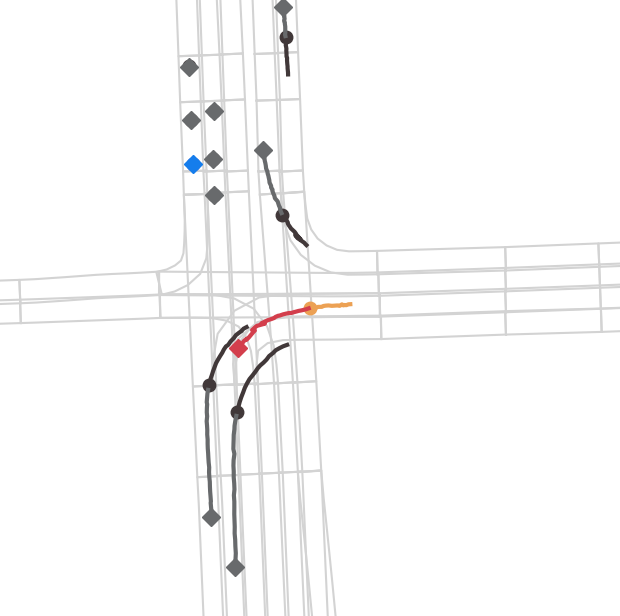
\includegraphics[width=0.23\linewidth]{chapter_6_Efficient_Baselines/qualitative_tits/val-120-general-view.png}} & 
		\fbox{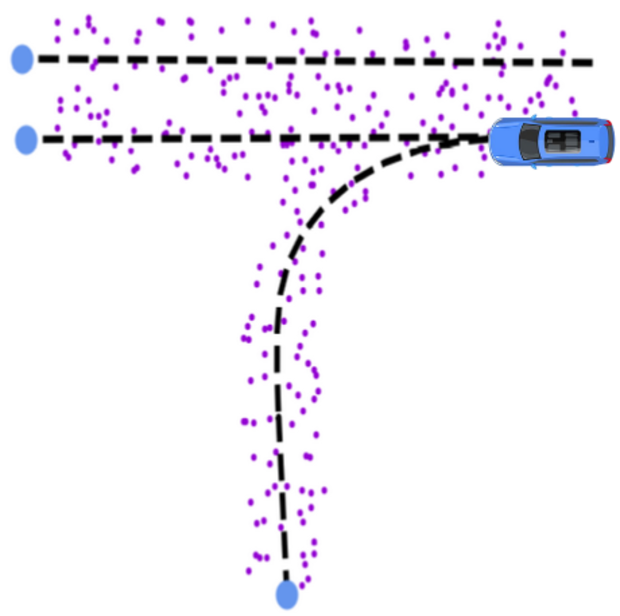
\includegraphics[width=0.23\linewidth]{chapter_6_Efficient_Baselines/qualitative_tits/val-120-plausible_hdmap.png}} &
		\fbox{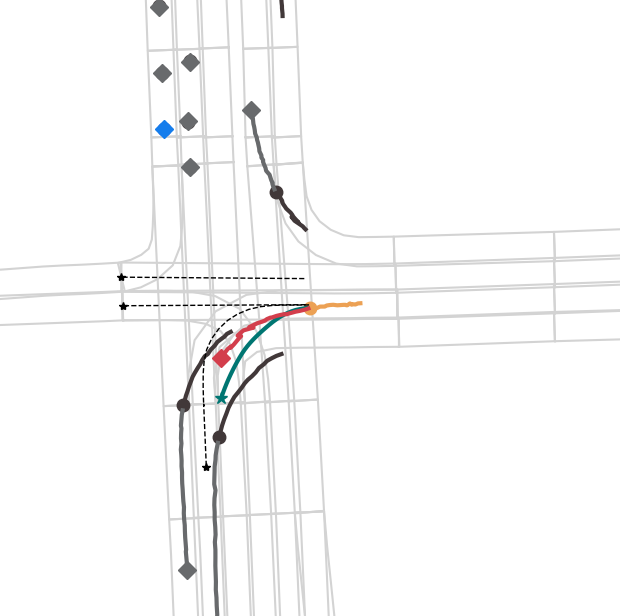
\includegraphics[width=0.23\linewidth]{chapter_6_Efficient_Baselines/qualitative_tits/val-120-unimodal.png}} & 
		\fbox{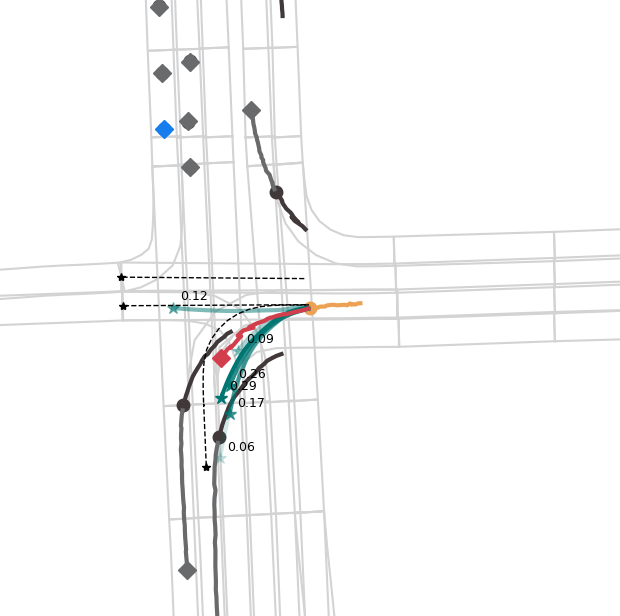
\includegraphics[width=0.23\linewidth]{chapter_6_Efficient_Baselines/qualitative_tits/val-120-multimodal_k_6.png}}
		
		\tabularnewline
		
		\fbox{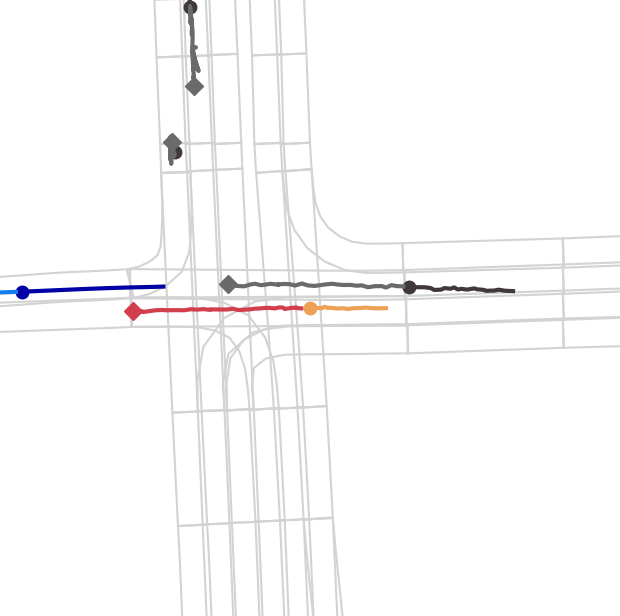
\includegraphics[width=0.23\linewidth]{chapter_6_Efficient_Baselines/qualitative_tits/val-215-general-view.png}} & 
		\fbox{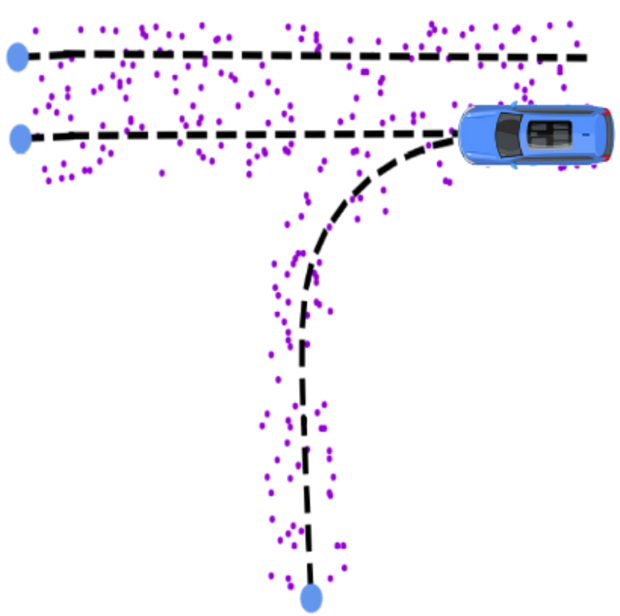
\includegraphics[width=0.23\linewidth]{chapter_6_Efficient_Baselines/qualitative_tits/val-215-plausible_hdmap.png}} &
		\fbox{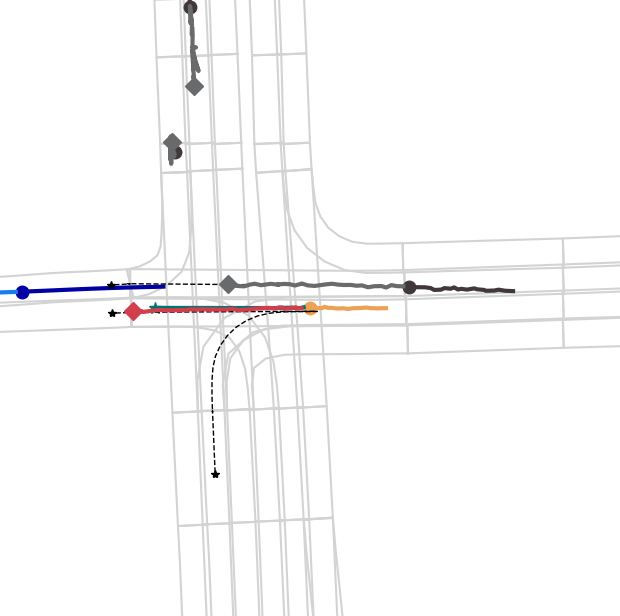
\includegraphics[width=0.23\linewidth]{chapter_6_Efficient_Baselines/qualitative_tits/val-215-unimodal.png}} & 
		\fbox{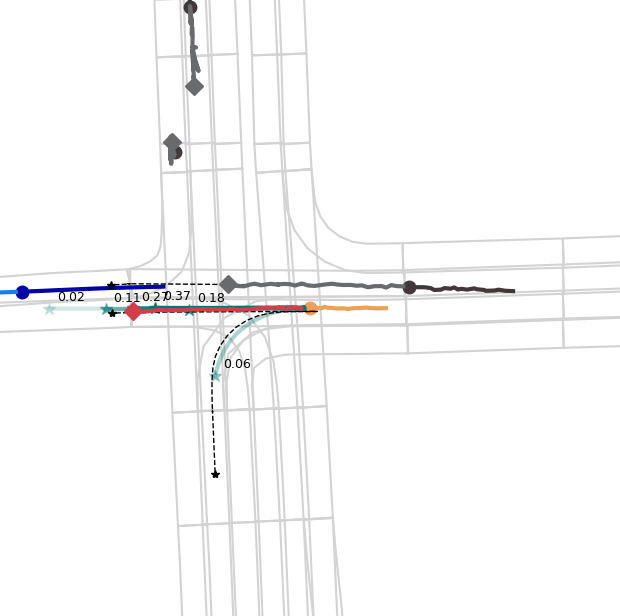
\includegraphics[width=0.23\linewidth]{chapter_6_Efficient_Baselines/qualitative_tits/val-215-multimodal_k_6.png}}
		
		\tabularnewline
		
		\fbox{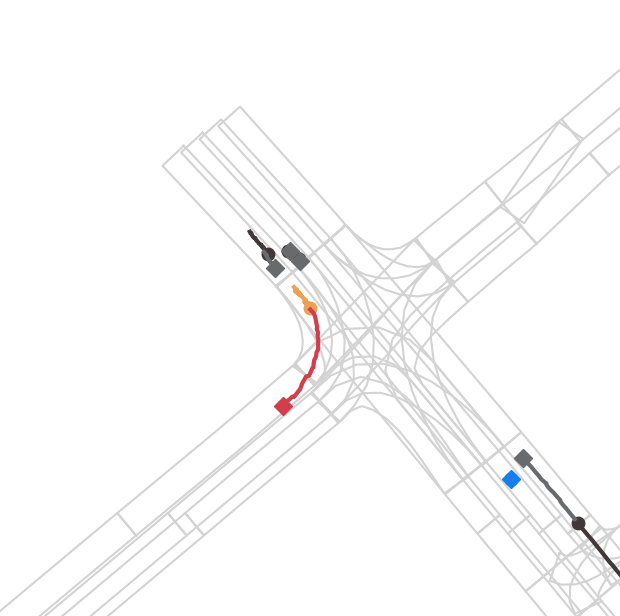
\includegraphics[width=0.23\linewidth]{chapter_6_Efficient_Baselines/qualitative_tits/val-205-general-view.png}} & 
		\fbox{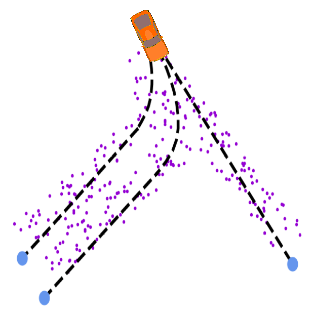
\includegraphics[width=0.23\linewidth]{chapter_6_Efficient_Baselines/qualitative_tits/val-205-plausible_hdmap.png}} &
		\fbox{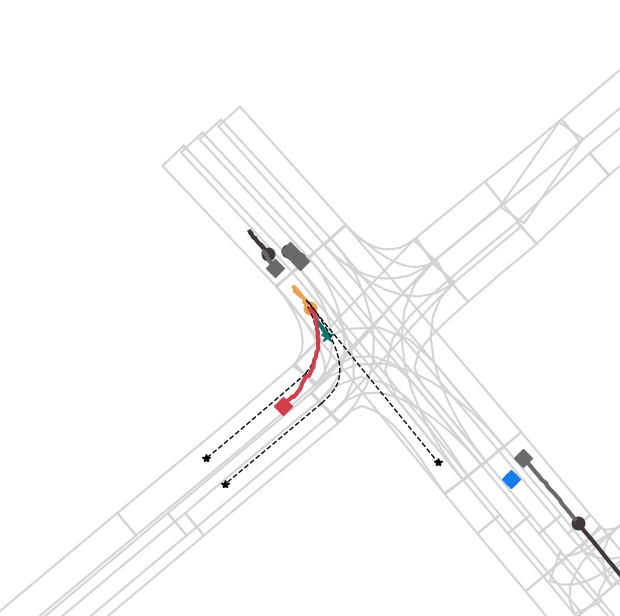
\includegraphics[width=0.23\linewidth]{chapter_6_Efficient_Baselines/qualitative_tits/val-205-unimodal.png}} & 
		\fbox{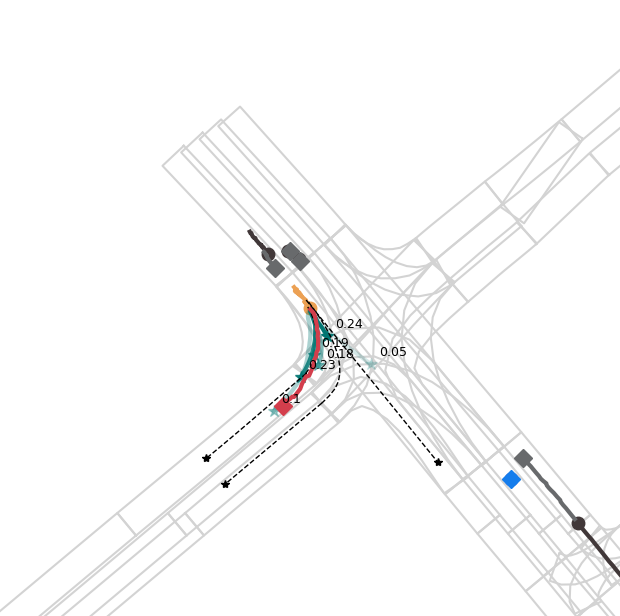
\includegraphics[width=0.23\linewidth]{chapter_6_Efficient_Baselines/qualitative_tits/val-205-multimodal_k_6.png}}
		
		\tabularnewline
		
		\fbox{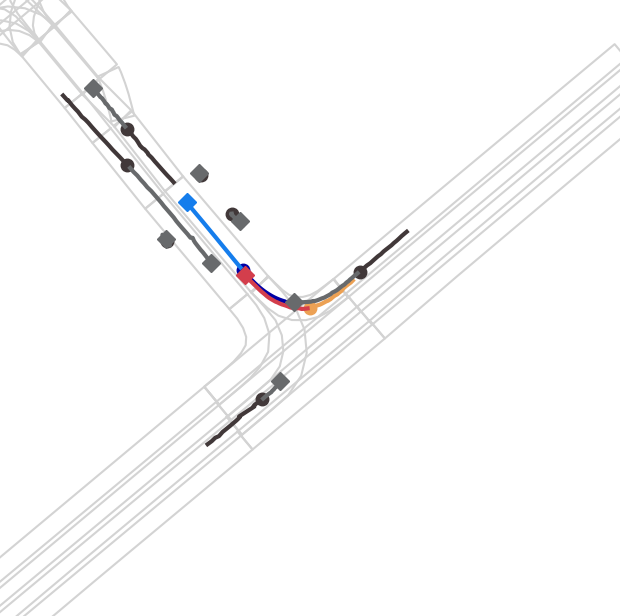
\includegraphics[width=0.23\linewidth]{chapter_6_Efficient_Baselines/qualitative_tits/val-152-general-view.png}} & 
		\fbox{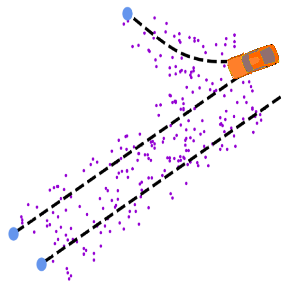
\includegraphics[width=0.23\linewidth]{chapter_6_Efficient_Baselines/qualitative_tits/val-152-plausible_hdmap.png}} &
		\fbox{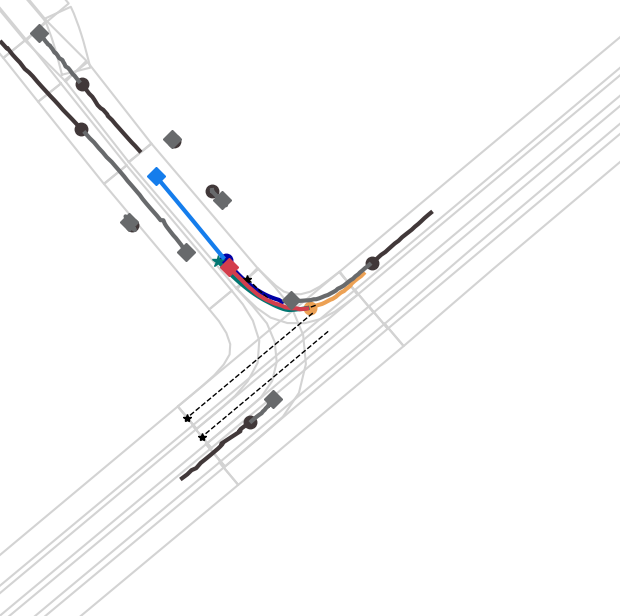
\includegraphics[width=0.23\linewidth]{chapter_6_Efficient_Baselines/qualitative_tits/val-152-unimodal.png}} & 
		\fbox{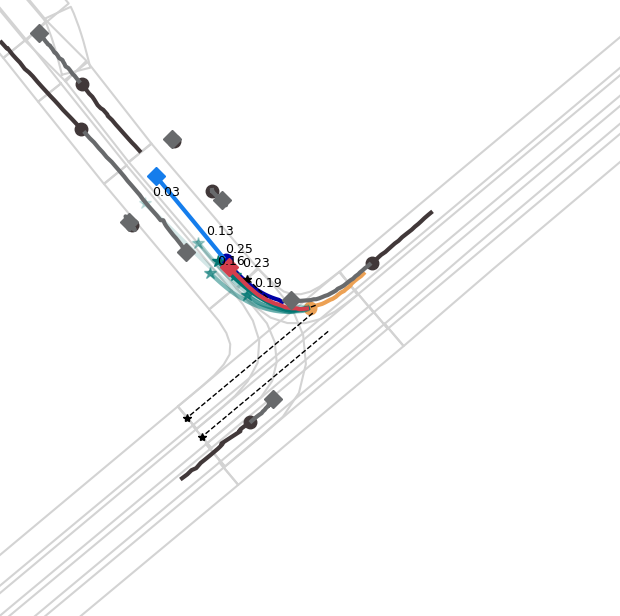
\includegraphics[width=0.23\linewidth]{chapter_6_Efficient_Baselines/qualitative_tits/val-152-multimodal_k_6.png}}
		
		\tabularnewline
		
		\fbox{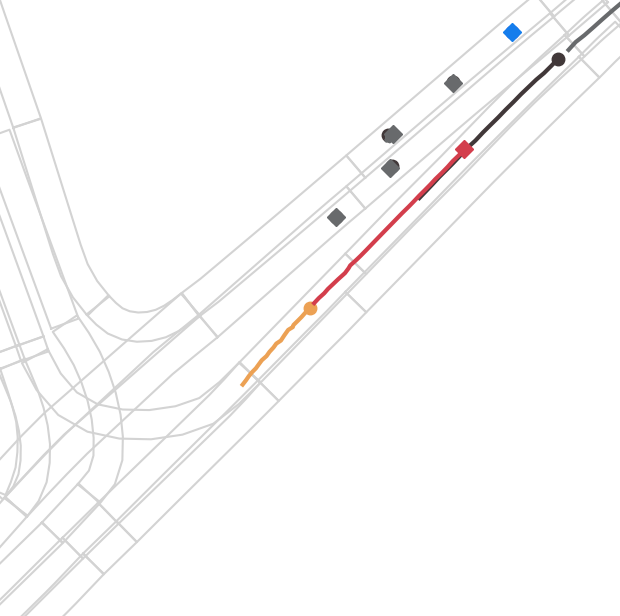
\includegraphics[width=0.23\linewidth]{chapter_6_Efficient_Baselines/qualitative_tits/val-209-general-view.png}} & 
		\fbox{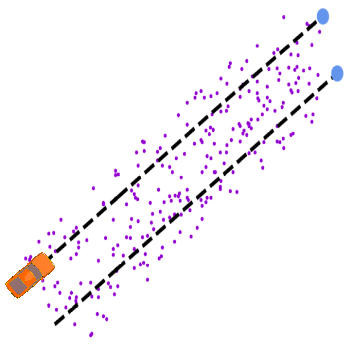
\includegraphics[width=0.23\linewidth]{chapter_6_Efficient_Baselines/qualitative_tits/val-209-plausible_hdmap.png}} &
		\fbox{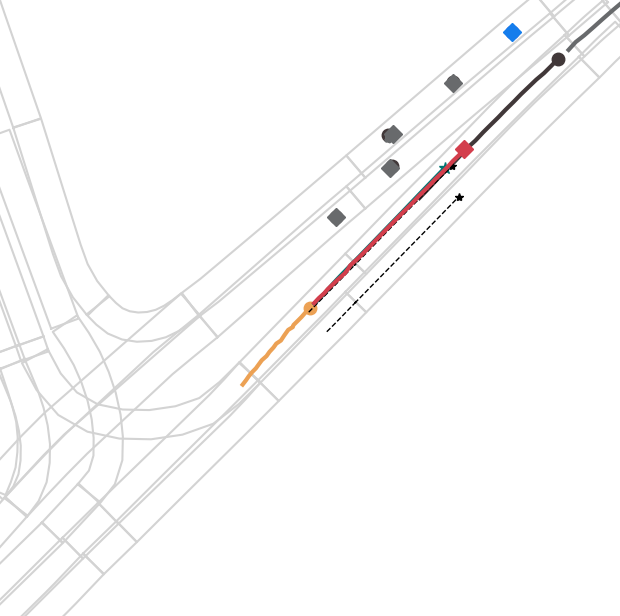
\includegraphics[width=0.23\linewidth]{chapter_6_Efficient_Baselines/qualitative_tits/val-209-unimodal.png}} & 
		\fbox{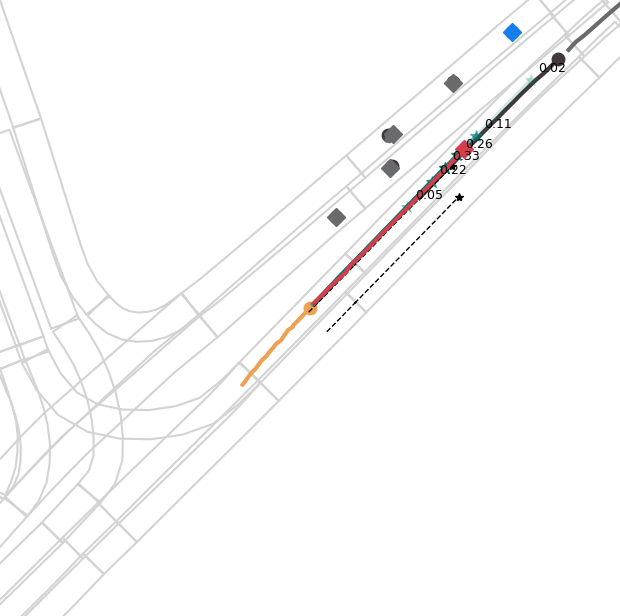
\includegraphics[width=0.23\linewidth]{chapter_6_Efficient_Baselines/qualitative_tits/val-209-multimodal_k_6.png}}
		
		\tabularnewline
		
		General view & Plausible HDMap & $k$=1 prediction & $k$=6 predictions \tabularnewline
	\end{tabular}
	\captionsetup{justification=justified}
	\caption[Qualitative Results on challenging scenarios in the Argoverse 1 validation set using our best model]{Qualitative Results on challenging scenarios in the Argoverse 1 validation set using our best model.	We represent: our vehicle (\textbf{\textcolor{blue}{ego}}), the \textbf{\textcolor{YellowOrange}{target agent}}, and \textbf{\textcolor{gray75}{other agents}}. We can also see the \textbf{\textcolor{red}{ground-truth}} trajectory of the target agent, our \textbf{\textcolor{ForestGreen}{multimodal predictions}} (with the corresponding confidences) and \textbf{plausible centerlines}. Circles represent last observations and diamonds last future positions. As we can see the plausible HDMap serves as a good guidance to our model, which can predict reasonable trajectories in presence of multiple agents and challenging scenarios. We show, from left to right, a general view of the traffic scenario (including social and map information), our calculated plausible HDMap, unimodal prediction (best mode in terms of confidence) and multimodal prediction (\textit{k} = 6), including confidences (the higher, the most probable)}
	\label{fig:chapter_6/argoverse_1_qualitative_results}
\end{figure}

\subsection{Efficiency discussion}
\label{subsec:6_efficiency_discussion}

In terms of \textbf{efficiency discussion}, to the best of our knowledge, very few methods reports efficiency-related information \cite{gilles2022gohome, gilles2021home, liu2021multimodal, gao2020vectornet}. Furthermore, comparing runtimes is difficult, as only a few competitive methods provide code and models. The Argoverse Benchmark~\cite{chang2019argoverse} provides insightful metrics about the model's performance, mainly related with the predictions error. However, there are no metrics about efficiency (\ie \ model complexity in terms of parameters or FLOPs). In the AD context, we consider these metrics as important as the error evaluation because, in order to design a reliable AD stack, we must produce reliable predictions on time, meaning the inference time (related to model complexity and inputs) is crucial. SOTA methods already provide predictions with an error lesser than 1 meter in the multi-modal case. In our opinion, an accident will rarely happen because some obstacle predictions are offset by one or half a meter, this uncertainty in prediction can be acceptable in the design of AV, but rather because lack of coverage or delayed response time. Despite its high accuracy and fast inference time, LaneGCN \cite{liang2020learning} makes use of multiple GNN layers that can lead to issues with over-smoothing for map-encoders \cite{li2018deeper}. Moreover, as mentioned in \cite{gao2020vectornet}, CNN-based models for processing the HD map information are able to capture social and map interactions, but most of them are computationally too expensive. LaneRCNN \cite{zeng2021lanercnn} adds huge number of hyperparameters to the model, making it quite complex since it proposes to capture agent and map interactions with a local interaction graph per agent, not just a single vector. 

\begin{table}[h]
	\centering
	\captionsetup{justification=justified}
	\caption[Efficiency comparison of our baselines against SOTA methods]{Efficiency comparison of our baselines against SOTA methods. We show the number of parameters for each model, FLOPs, minADE (k=6) in the Argoverse test set, and runtime. Works from \cite{gao2020vectornet} focus on unimodal predictions (k=1). \textit{N/A} stands for \textit{Not Available}. Time measured on a RTX 2080 Ti (using batch 32). Some numbers are borrowed from \cite{zhou2022hivt, bhattacharyya2023ssl}.
	}
	\resizebox{\linewidth}{!}{
		\begin{tabular}{lcccc}
			\toprule
			Model & \# Par.~(M) & FLOPs (G)~$\downarrow$ & minADE~(m) $\downarrow$ & Run~(ms) $\downarrow$ \\
			\midrule
			CtsConv~\cite{walters2020trajectory} & 1.08 & 0.34 & 1.85 & 684  \\
			%$\rho_1$-ECCO~\cite{walters2020trajectory} & 0.051 & 1.7 & 3.89 \\
			%mmTransformer~\cite{liu2021mmtransf} & 4 & 1.77 & & 0.66 \\
			R18-k3-c1-r100~\cite{gao2020vectornet} & 0.25 & 0.66 & 2.21 & \textit{N/A} \\
			R18-k3-c1-r400~\cite{gao2020vectornet} & 0.25 & 10.56 & 2.16 & \textit{N/A} \\
			VectorNet~\cite{gao2020vectornet} & \textbf{0.072} & 0.41 & 1.66 & 1103 \\
			DenseTNT (w/ 100ms opt.) \cite{gu2021densetnt} & 1.1 & 0.763 & 0.88 & 2644 \\
			DenseTNT (w/ goal set pred.) \cite{gu2021densetnt} & 1.1 & 0.763 & 0.85 & 531 \\
			LaneGCN \cite{liang2020learning} & 3.7 & 1.071 & 0.87 & 173 \\
			mmTransformer \cite{liu2021multimodal} & 2.607 & 0.177 & 0.84 & \textit{N/A} \\
			MF-Transformer \cite{he2022multi} & 2.469 & 0.408 & \textbf{0.82} & \textit{N/A} \\
			HOME+GOHOME~\cite{gilles2022gohome} & 0.40 & 0.09 & 0.94 & 32 \\
			\midrule
			% OURS
			% GAN-based 
			% MAPFE4MP (Social baseline) \cite{gomez2022exploringmapbased} & 0.105 & \textbf{0.007} & 1.26 & 7 \\
			% MAPFE4MP (Map baseline) \cite{gomez2022exploringmapbased} & 0.621 & 0.047 & 0.96 & 31 \\
			
			Ours & 1.235 & \textbf{0.038} & 0.91 & \textbf{16} \\
			\bottomrule
	\end{tabular}}
	\label{table:6_argoverse_1_efficiency_comparison}
\end{table}

Similar to image classification, where model efficiency depends on its accuracy and parameters/\acp{FLOP}, we use the same criteria to compare models. We show the \textbf{efficiency comparison} with other relevant methods in Table \ref{table:6_argoverse_1_efficiency_comparison}. Some minor operations were not supported, yet, their contributions to the number of \acp{FLOP} were residual and ignored. The results for the other methods are consulted from \cite{gilles2021home} \cite{gilles2022gohome} \cite{gao2020vectornet} \cite{he2022multi}. We calculate \acp{FLOP} (assuming the relation: $\text{GMACs} \approx 0.5 * \text{GFLOPs}$) and parameters using a third-party library \footnote{https://github.com/facebookresearch/fvcore}.

In order to calculate the FLOPs, we follow the common practice \cite{gao2020vectornet} \cite{gu2021densetnt} \cite{gilles2022gohome} of fixing the number of lanes \ie \ the number of centerlines is limited to 3. %, since we focus on the plausible area around the target agent.
% 40 and 10 the number of lanes (if the method is based on polyline or GNN, not raster) and agents per traffic scenario, respectively.
%
\cite{gao2020vectornet} compares its GNN backbone with CNNs of different kernel sizes and map resolution to compute deep map features (decoder operations and parameters are excluded, min), demonstrating how CNN based methods noticeably increase the amount of parameters and operations per second. We do not require CNNs to extract features from the HD map since we use our map-based feature extractor to obtain the feasible area (see Section \ref{subsec:6_efficient_baselines_map_baseline}), assuming anisotropic driving (the most important features are ahead) and non-holonomic constraints, in such a way these features are interpretable in comparison with CNNs high-dimensional outputs. Note that, in both variants (social and map baselines), the self-attention module is used with a dynamic number of input agents, this typically implies a quadratic growth in complexity with the number of agents in the scene~\cite{vaswani2017attention}, yet, this only applies to the MHSA layers.

Even though our methods do not obtain the best regression metrics, we achieve up-to-pair results (Table \ref{table:6_argoverse_1_efficiency_comparison}) against other SOTA approaches whilst our number of FLOPs is several orders of magnitude smaller than other approaches \cite{gu2021densetnt} \cite{liang2020learning}, obtaining a good trade-off (specially the map baseline) between model complexity and accuracy (minADE, k=6), making it suitable for real-time operation in the field of AD. In our case, considering the top-25 regression metrics we achieve near SOTA results (just 15 cm, which represents 18.5 \%, worse in terms of minADE k=6 regarding our final approach) while achieving an impressive reduction of parameters and FLOPs. As observed in Table \ref{table:6_argoverse_1_efficiency_comparison}, if we compare our final model, which includes social information, agents interaction and preliminary road information, and the methods with the closest minADE k=6 [m] (LaneGCN \cite{liang2020learning}, HOME \cite{gilles2021home} and GOHOME \cite{gilles2022gohome}), we obtain a reduction of 96 \%, 99 \% and 48 \% respectively in terms of FLOPs. It can be observed how including preliminary road information assuming non-holonomic \cite{triggs1993motion} and anisotropic \cite{ross1989planning} constraints respectively (that is, we mostly focus on the front driveable area) instead of processing the whole map, as well as computing social interactions via graph convolutional networks, boost our model for further integration edge-computing devices with a minimum accuracy loss acceptable for real-world Autonomous Driving applications.

% Even though our method do not obtain the best regression metrics, we achieve comparable results (Table \ref{table:effcomp}) against other SOTA approaches whilst our number of FLOPs is several orders of magnitude smaller than other approaches \cite{gu2021densetnt} \cite{liang2020learning}, obtaining a good trade-off between model complexity and error (minADE, k=6).

Moreover, as it is well known in machine learning, the number of parameters is not always proportional to the inference speed. In that sense, our transformer approach also has certain benefits in comparison to LSTM/RNN temporal encoding, since these are non-parallelizable, therefore, despite having more parameters, transformers are faster~\cite{vaswani2017attention}.

\section{Summary}
\label{sec:6_summary}

In this Chapter, we propose several efficient baselines, progressively aggregating contextual information from social info to augmented map via a transformer-based model that does not rely on heavily annotated HD maps, yet it uses past trajectories and minimal map priors.
%
The final proposed method combines the transformer attention mechanisms with GNNs to model agent interactions. We show that it has less parameters than other methods, and it is faster than most previous methods. We achieve near-SOTA results on the Argoverse Motion Forecasting Benchmark while having a low computational cost compared to other state-of-the-art proposals. In future works, we plan to extend our work for multi-agent modal prediction in the Argoverse 2 dataset, taking into account more complex features and interactions in an efficient and powerful way.Our framework is open-sourced.